
\documentclass[12pt, a4paper]{report}
\usepackage{epsfig}
\usepackage{subfigure}
%\usepackage{amscd}
\usepackage{amssymb}
\usepackage{graphicx}
%\usepackage{amscd}
\usepackage{amssymb}
\usepackage{subfiles}
\usepackage{framed}
\usepackage{subfiles}
\usepackage{amsthm, amsmath}
\usepackage{amsbsy}
\usepackage{framed}
\usepackage[usenames]{color}
\usepackage{listings}
\lstset{% general command to set parameter(s)
	basicstyle=\small, % print whole listing small
	keywordstyle=\color{red}\itshape,
	% underlined bold black keywords
	commentstyle=\color{blue}, % white comments
	stringstyle=\ttfamily, % typewriter type for strings
	showstringspaces=false,
	numbers=left, numberstyle=\tiny, stepnumber=1, numbersep=5pt, %
	frame=shadowbox,
	rulesepcolor=\color{black},
	,columns=fullflexible
} %
%\usepackage[dvips]{graphicx}
\usepackage{natbib}
\bibliographystyle{chicago}
\usepackage{vmargin}
% left top textwidth textheight headheight
% headsep footheight footskip
\setmargins{3.0cm}{2.5cm}{15.5 cm}{22cm}{0.5cm}{0cm}{1cm}{1cm}
\renewcommand{\baselinestretch}{1.5}
\pagenumbering{arabic}
\theoremstyle{plain}
\newtheorem{theorem}{Theorem}[section]
\newtheorem{corollary}[theorem]{Corollary}
\newtheorem{ill}[theorem]{Example}
\newtheorem{lemma}[theorem]{Lemma}
\newtheorem{proposition}[theorem]{Proposition}
\newtheorem{conjecture}[theorem]{Conjecture}
\newtheorem{axiom}{Axiom}
\theoremstyle{definition}
\newtheorem{definition}{Definition}[section]
\newtheorem{notation}{Notation}
\theoremstyle{remark}
\newtheorem{remark}{Remark}[section]
\newtheorem{example}{Example}[section]
\renewcommand{\thenotation}{}
\renewcommand{\thetable}{\thesection.\arabic{table}}
\renewcommand{\thefigure}{\thesection.\arabic{figure}}
\title{Research notes: linear mixed effects models}
\author{ } \date{ }


\begin{document}
	\author{Kevin O'Brien}
	\title{Mixed Models for Method Comparison Studies}
	\tableofcontents
	

	
	%	
	%	\citet{schabenberger} describes the examination of model-data agreement as comprising several elements; \begin{itemize}
	%		\item residual analysis,
	%		\item goodness of fit,
	%		\item collinearity diagnostics
	%		\item influence analysis.
	%	\end{itemize}
	%	
	%\end{abstract}
	\chapter{Residual Analysis and Influence Diagnostics for Method Comparison}
	Model validation and model appraisal are vital parts of the modelling process, yet are too often overlooked. Using a small set of simple measures and methods, such as the AIC and $R^2$ measures, is insufficient to properly assess the usefulness of a fitted model. In classical linear models model diagnostics are now considered a required part of any statistical analysis, and the methods are commonly available in statistical packages and standard textbooks on applied regression. A full and comprehensive
	analysis that comprises residual analysis and influence analysis for testing model assumptions, should be carried out. However it has been noted by several papers \citep{Christensen, schabenberger} that model diagnostics do not often accompany LME model analyses. Furthermore, a suite of dagnostic procedures designed for method comparison should be adopted.
	
	
	\section{Influence Diagnostics}
	Model diagnostic techniques can determine whether or not the distributional assumptions are satisfied, but also to assess the influence of unusual observations. Following model specification and estimation, it is of interest to explore the model-data agreement by raising pertinent questions. \citet{pb} provide some insight into how to compute and interpret model diagnostic plots for LME models. Unfortunately this aspect of LME theory is not as expansive as the corresponding body of work for Linear Models. Their particular observations will be reverted to shortly. Further to the analysis of residuals, \citet{schabenberger} recommends the examination of the following questions:
	\begin{itemize}
		\item Does the model-data agreement support the model assumptions?
		\item Should model components be refined, and if so, which components? For example, should certain explanatory variables
		be added or removed, and is the covariance of the observations properly specified?
		\item Are the results sensitive to model and/or data? Are individual data points or groups of cases particularly
		influential on the analysis?
	\end{itemize}
	
	The last of these three questions, regarding influential points, is of particular interest in the context of Method Comparison. After fitting an LME model, it is important to carry put model diagnostics to check whether distributional assumptions for the residuals as satisfied and whether the fit the model is sensitive to unusual assumptions. The process of carrying out model
	diagnostic involves several informal and formal techniques, which will mentioned throughout the chapter.
	
	Influential points have a large influence on the fit of the model. Influential points are a set of one or more observations whose removal would cause a different conclusion in the analysis, e.g. substantially changes the estimate of the regression coefficients. \citet{west} remarks that influence diagnostics play an important role in the interpretation of results, because influential data can negatively influence the statistical model and generalizability of the model. \citet{schabenberger} remarks that the concept of critiquing the model-data agreement applies in mixed models in the same way as in linear
	fixed-effects models. In fact, because of the more complex model structure, you can argue that model and
	data diagnostics are even more important \citep{west}.
	%Influential points have a large influence on the fit of the model. 
	
	%One approach for determining influential points is to compare the fit of the model with and without each observation.
	
	%The basic rationale behind identifying influential data is that when iteratively single units are omitted from the data, models based on these data should not produce substantially different estimates. 
	
	

	\chapter{Residual Analysis and Influence Diagnostics for Method Comparison}
%	Model validation and model appraisal are vital parts of the modelling process, yet are too often overlooked. Using a small handful of simple measures and methods, such as the AIC and $R^2$ measures, is insufficient to properly assess the usefulness of a fitted model. 
	

 In classical linear models model diagnostics are now considered a required part of any statistical analysis, and the methods are commonly available in statistical packages and standard textbooks on applied regression. However it has been noted by several papers \citep{Christensen, schabenberger} that model diagnostics do not often accompany LME model analyses. Well established methods are commonly available in statistical packages and standard textbooks on applied regression. However it has been noted by several papers that model diagnostics do not often accompany LME model analyses. 

A comprehensive analysis that comprises residual analysis and influence analysis for testing model assumptions, should be carried out. 
	
	Following model specification and estimation, it is of interest to explore the model-data
	agreement by raising pertinent questions. Pinheiro and Bates provide some insight into how to compute and interpret model diagnostic plots for LME models. Unfortunately this aspect of LME theory is not as expansive as the corresponding body of work for linear models. Their particular observations will be reverted to shortly. 
	
\citet{schabenberger} discusses the state of LME diagnostics tools, providing a useful summary of established measures. Further to the analysis of residuals, \citet{schabenberger} recommends the examination of the following questions:
\newpage
Model diagnostics techniques determine whether or not the distributional assumptions are satisfied, and to assess the influence of unusual observations, and have been become a required part of any statistical analysis. Well established methods are commonly described and implemented available on standard statistics textbooks, and implemented in software packages. However it has been noted by several papers that model diagnostics do not often accompany LME model analyses. \citet{schabenberger} discusses the state of LME diagnostics tools, providing a useful summary of established measures.
	
	A full and comprehensive
	analysis that comprises residual analysis and influence analysis for testing model assumptions, should be carried out.  In classical linear models model diagnostics are now considered a required part of any statistical analysis, and the methods are commonly available in statistical packages and standard textbooks on applied regression. However it has been noted by several papers \citep{Christensen, schabenberger} that model diagnostics do not often accompany LME model analyses.
	
Following model specification and estimation, it is of interest to explore the model-data agreement by raising pertinent questions.  Further to the analysis of residuals, \citet{schabenberger} recommends the examination of the following questions:

\citet{PB} provide some insight into how to compute and interpret model diagnostic plots for LME models. Unfortunately this aspect of LME theory is not as expansive as the corresponding body of work for linear models.

Influential points are of particular interest in the context of method comparison. After fitting an LME model, it is important to carry put model diagnostics to check whether distributional assumptions for the residuals as satisfied and whether the fit the model is sensitive to unusual assumptions. \citet{schabenberger} remarks that the concept of critiquing the model-data agreement applies in LME models in the same way as in linear fixed-effects models. \citet{west} argues that model and data diagnostics are even more important because of the more complex model structure,.


%http://www.itl.nist.gov/div898/handbook/pmd/section4/pmd44.htm



	
\section{Residual Analysis}
As with classical models, there are two key techniques for LME models: a residual plot and the normal probability plot. The rationale is that, if the model is properly fitted to the model, then the residuals would approximate the random errors that one should expect.
If the residuals behave randomly, with no discernible trend, the model has fitted the data well. Conversely, if some sort of non-random trend is evident in the model, then the model can be considered to be poorly fitted. 

The underlying assumptions for LME models are similar to those of classical linear models. However, for LME models the matter of residuals are more complex, both from a theoretical point of view and from the practicalities of implementing a comprehensive analysis using statistical software. \citet{schabenberger} discusses residuals for LME model, providing a useful summary of various techniques. Prominent in literature is the taxonomy of residuals for LME Models, distinguishing between condition residuals, marginal residuals and EBLUPS, including \citet{hildenminton, schabenberger, west, NobreSinger2007}.  

Statistical software environments, such as the \texttt{R} programming language, provides a suite of tests and graphical procedures for appraising a fitted LME model, with several of these procedures analysing the model residuals. Texts such as \citet{PB,west,Galecki} describe what can be implemented for LME residual analyses with statistical software, such as \texttt{R} and \texttt{SAS}.


In the context of method comparison, a residual analysis would be carried out just as any other LME model would, testing normality. There is little scope for adding additional insights, other than to say that it is possible to create plots specific to each method. The figures on the next page depict the residual analysis for the \textit{Blood} data, which can be used to indicate which methods disagree with the rest, but these would be a confirmation of something detected previously.

	
Analysis of the residuals could determine if the methods of measurement disagree systematically, or whether or not erroneous measurements associated with a subset of the cases are the cause of disagreement. 
The figure depicts residual plot for the systolic blood pressure example used in \citet{BA99}. Points are labelled by subjects, with cases 67, 68 and 71 being among the prominent cases. Prominent cases warrant further investigation, but an analyst should procede to influence diagnostics beforehand.

\subsubsection{LME Residual Analysis}
\begin{figure}[h!]
	\centering
	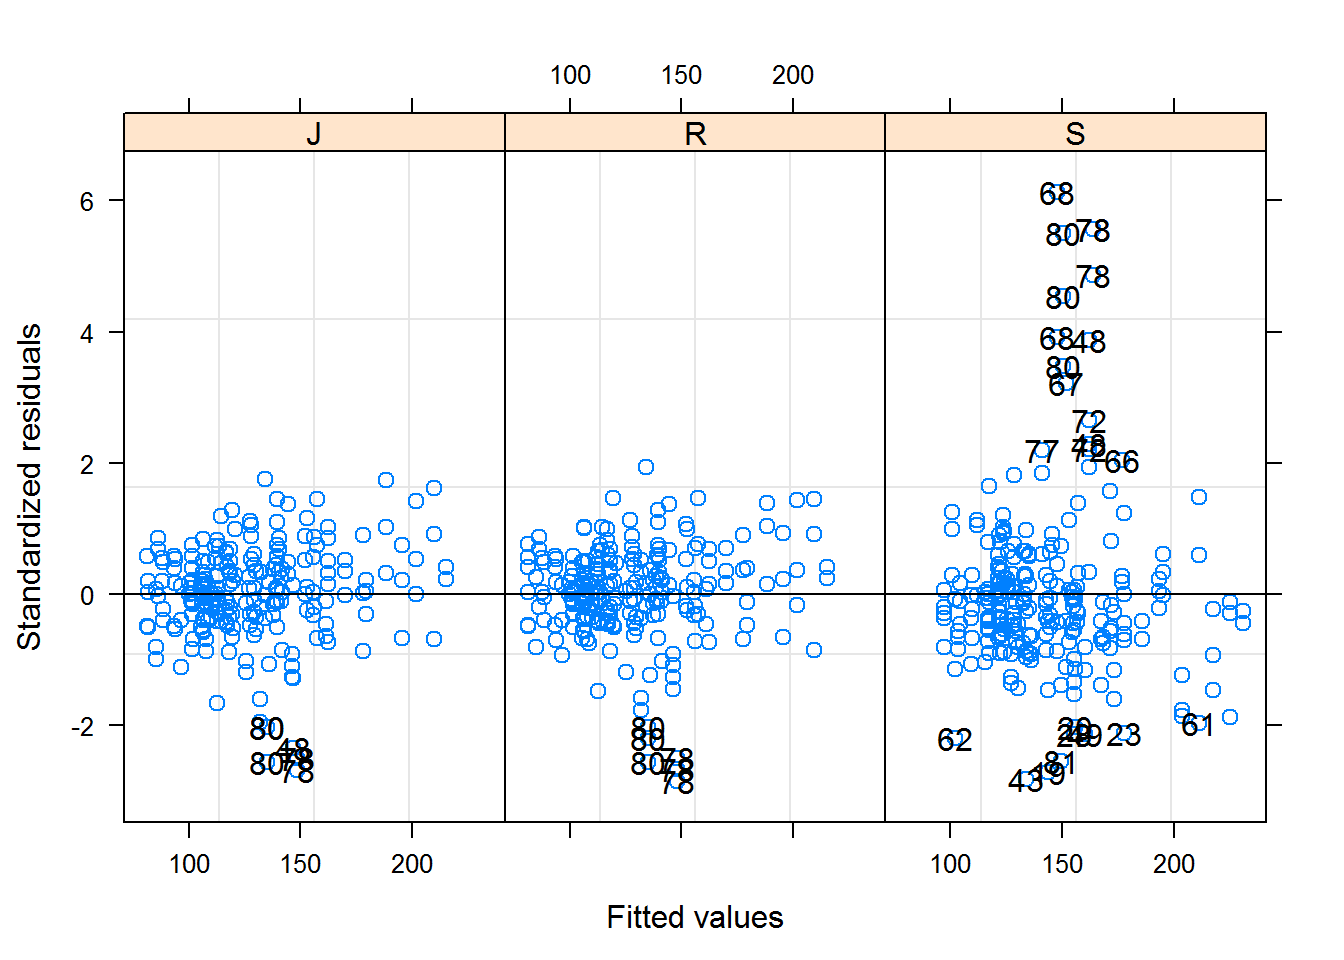
\includegraphics[width=0.7\linewidth]{images/bloodnlme-ResidPlot}
	\caption{LME Residuals by Method (Blood Pressure Data)}
\end{figure}



Residual analysis is a widely used model validation technique. A residual is simply the difference between an observed value and the corresponding fitted value, as predicted by the model.  Residuals are used to examine model assumptions and to detect outliers and potentially influential data point. 

As with classical models, there are two key techniques: a residual plot and the normal probability plot. The rationale is that, if the model is properly fitted to the model, then the residuals would approximate the random errors that one should expect.

For classical analyses, residual diagnostics are typically implemented as a plot of the observed residuals and the predicted values. A visual inspection for the presence of trends inform the analyst on the validity of distributional assumptions, and to detect outliers and influential observations. 
	
However, for LME models the matter of residual is more complex, both from a theoretical point of view and for implementing a comprehensive analysis using statistical software. As the LME model can be tailored to the needs of the particular research question, the rationale behind the model appraisal must follow accordingly.
	
\citet{schabenberger} discusses residuals for LME model, providing a useful summary of various techniques. Prominent in literature is the taxonomy of residuals for LME Models, distinguishing between condition residuals, marginal residuals and EBLUPS, including \citet{ HildenMinton, schabenberger, west, NobreSinger2011}. The underlying assumptions for LME models are similar to those of classical linear models. 
	
Statistical software environments, such as the \texttt{R} Programming language, provides a suite of tests and graphical procedures for appraising a fitted linear model, with several of these procedures analysing the model residuals. Texts such as \citet{PB,west,Galecki} describe what can be implemented for LME residual analyses with statistical software, such as \texttt{R} and \texttt{SAS}.
	
\subsection{Residual Analysis for MCS}	
In the context of method comparison, a residual analysis would be carried out just as any other LME model would, testing normality. As such there is little scope for adding additional insights, other than to say that it is possible to create plots specific to each method. 
	
Analysis of the residuals could determine if the methods of measurement disagree systematically, or whether or not erroneous measurements associated with a subset of the cases are the cause of disagreement. 


\subsubsection{LME Residual Analysis}
However, for LME models the matter of residual is more complex, both from a theoretical point of view and from the practical matter of implementing a comprehensive analysis using statistical software. \citet{schabenberger} discusses residuals for LME model, providing a useful summary of various techniques. Prominent in literature is the taxonomy of residuals for LME models, distinguishing between condition residuals, marginal residuals and EBLUPS, including \citet{hildenminton, schabenberger, west, nobresinger2007}. The underlying assumptions for LME models are similar to those of classical linear models. 
	

For classical analysese, residual diagnostics are typically implemented as a plot of the observed residuals and the predicted values. A visual inspection for the presence of trends inform the analyst on the validity of distributional assumptions, and to detect outliers and influential observations. Diagnostics plots for the systolic blood pressure are featured in figure~\ref{fig:ResidPlot}
	
\begin{figure}[h!]
	\centering
	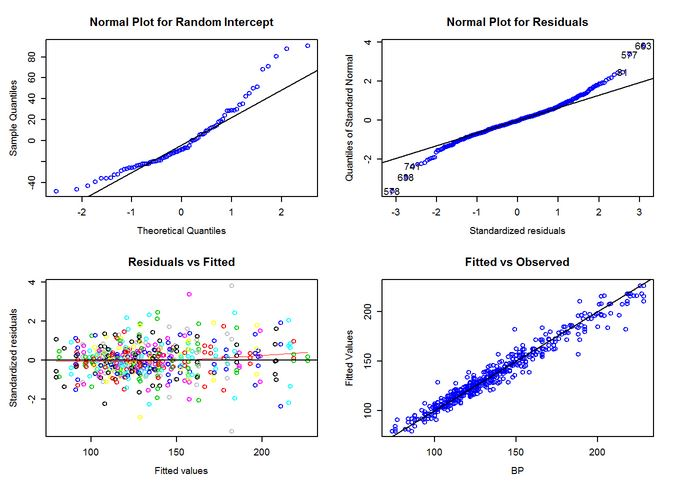
\includegraphics[width=0.9\linewidth]{images/ResidPlot}
	\caption{}
	\label{fig:ResidPlot}
\end{figure}

As the LME model can be tailored to the needs of the particular research question, the rationale behind the model appraisal must follow accordingly. 
For method comparison studies, one can create plots specific to each method, useful in determining which methods disagree with the rest.
 	
	
%	In the context of method comparison, a residual analysis would be carried out just as any other LME model would, testing normality. As such there is little scope for adding additional insights, other than to say that
%	it is possible to create plots specific to each method. The figures on the next page depict the residual analysis for the Blood data. This can be used to indicate which methods disagree with the rest, but these would be a confirmation of something detected previously.

%	\begin{figure}[h!]
%		\centering
%		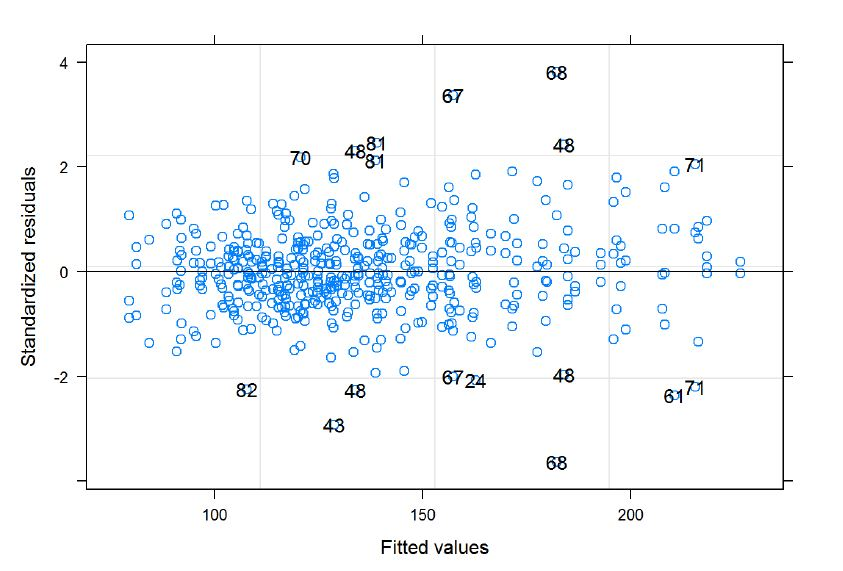
\includegraphics[width=0.8\linewidth]{images/Residuals-JS-Roy}
%	\end{figure}
	

The next figure depicts residual plot for the Systolic Blood Pressure example, panelled by the various measurement methods. It serves to confirm agreement between methods J and R, with lack of agreement between those two methods and method S. However, little insight can be gained as to what actually causes lack of agreement here. 

\begin{figure}[h!]
		\centering
		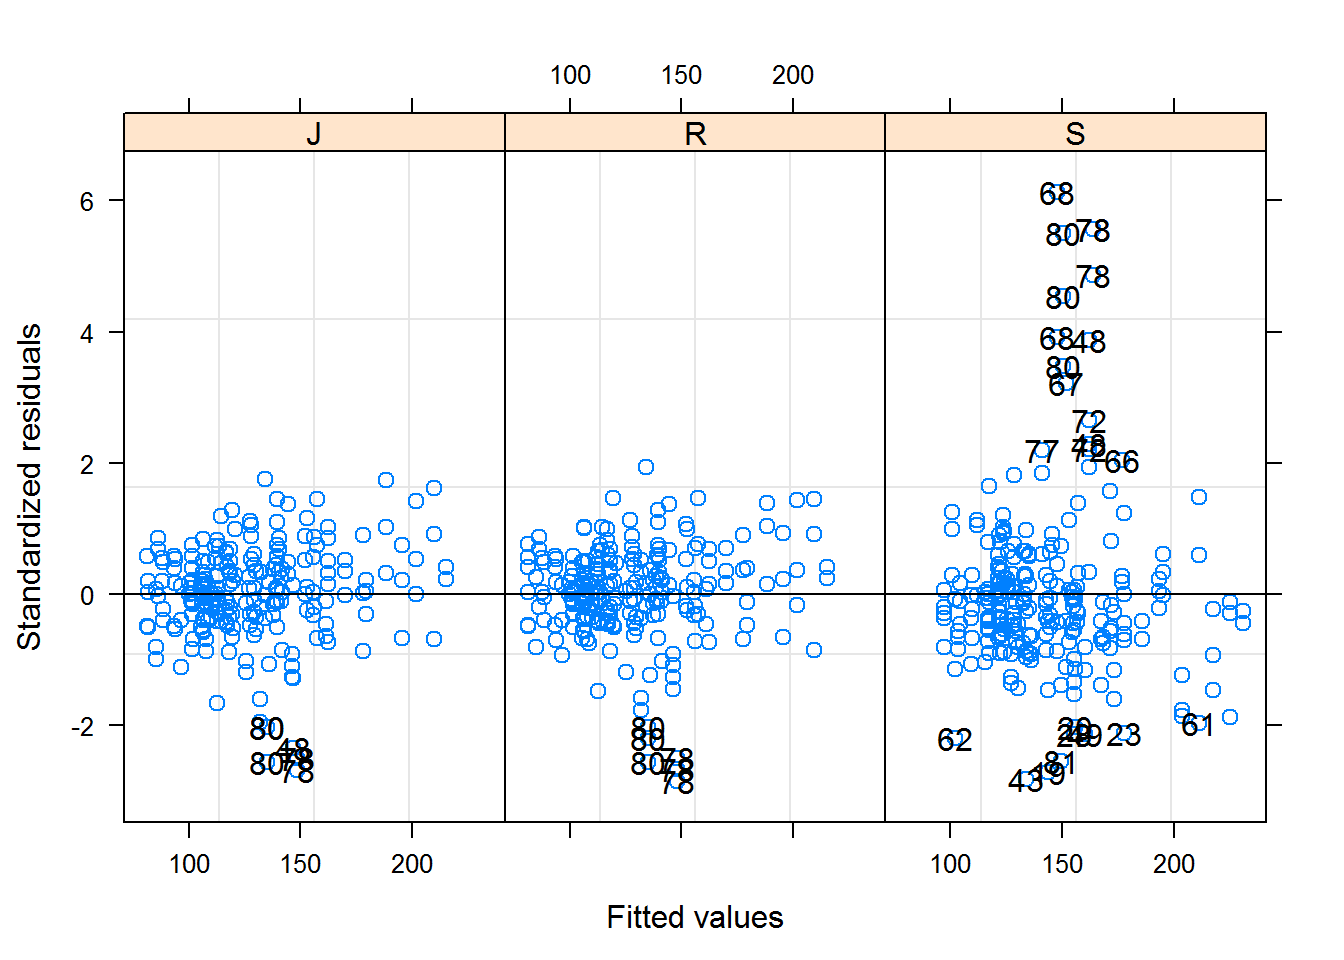
\includegraphics[width=0.8\linewidth]{images/bloodnlme-ResidPlot}
		\caption{LME Residuals by Method (Blood Pressure Data)}
\end{figure}


	
	%% \subsubsection{Why Use Residuals?}
	%If the model fit to the data were correct, the residuals would approximate the random errors that make the relationship between the explanatory variables and the response variable a statistical relationship. Therefore, if the residuals appear to behave randomly, it suggests that the model fits the data well. On the other hand, if non-random structure is evident in the residuals, it is a clear sign that the model fits the data poorly. The subsections listed below detail the types of plots to use to test different aspects of a model and give guidance on the correct interpretations of different results that could be observed for each type of plot.
	%------------------------------------------------------------------------------------------------------------------------ %

The underlying assumptions for LME models are similar to those of classical linear mdoels. There are two key techniques: a residual plot and the normal probability plot. Using the nlme package it is possible to create plots specific to each method. This is useful in determine which methods disagree with the rest.

Analysis of the residuals would determine if the methods of measurement disagree systematically, or whether or not erroneous measurements associated with a subset of the cases are the cause of disagreement. Erroneous measurements are incorrect measurements that indicate disagreement between methods that would otherwise be in agreement.
	%======================================================== %
	Once the residuals are computed, they can be used to make an assessment about the model fit. For LME models, we can plot the residuals against the fitted values, to assess the assumption of constant variance. 
	%	\begin{figure}[h!]
	%		\centering
	%		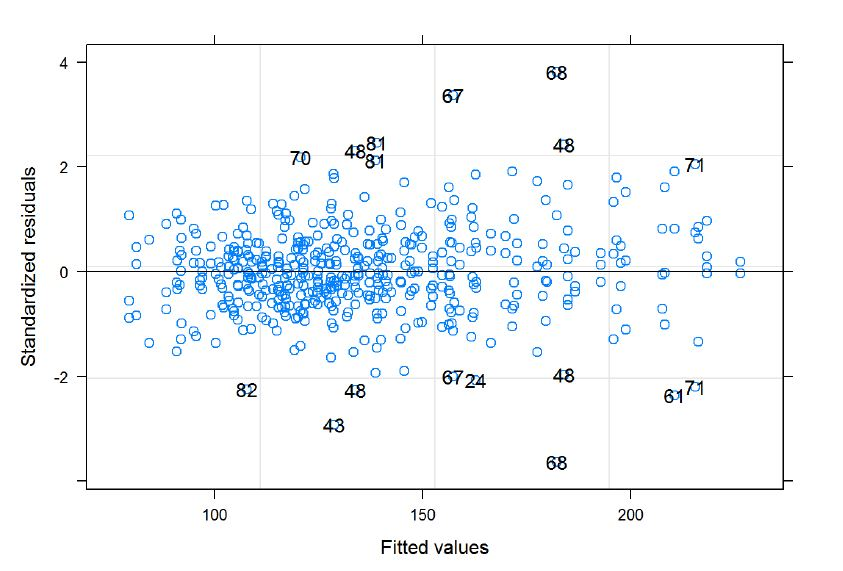
\includegraphics[width=0.9\linewidth]{images/Residuals-JS-Roy}
	%		\caption{}
	%		\label{fig:Residuals-JS-Roy}
	%	\end{figure}
	
	Normal probability plots can be rendered for each level of the random effects.  LME models assume that not only the within-cluster residuals are normally distributed, but that each level of the random effects are as well. LME models assume that the residuals of the model are normally distributed.  The residuals can be divided according to groups according to the method of measurement. In the following examples, we seperately assess normality the \textit{J} method residuals (the first 255 residuals) and \textit{S} method residuals (the remaining 255). Importantly the residuals from the \textit{J} method are normally distributed, but there is non-normality of the residuals according to the \textit{S} method.
	

	
	%
	%\subsubsection{Introduction}
	%In statistics and optimization, statistical errors and residuals are two closely related and easily confused measures of the deviation of an observed value of an element of a statistical sample from its "theoretical value". The error (or disturbance) of an observed value is the deviation of the observed value from the (unobservable) true function value, while the residual of an observed value is the difference between the observed value and the estimated function value.
	%
	%The distinction is most important in regression analysis, where it leads to the concept of studentized residuals.
	%
	%
	
	
	
	
	%		\begin{framed}
	%			\begin{verbatim}
	%			par(mfrow=c(1,2))
	%			qqnorm((resid(JS.roy1)[1:255]),
	%			pch="*",col="red",
	%			ylim=c(-40,40),
	%			main="Method J")
	%			qqline(resid(JS.roy1)[1:255],col="blue")
	%			qqnorm((resid(JS.roy1)[256:510]),
	%			pch="*",col="red",
	%			ylim=c(-40,40),
	%			main="Method S")
	%			qqline(resid(JS.roy1)[256:510],col="blue")
	%			par(mfrow=c(1,1))
	%			\end{verbatim}	
	%		\end{framed}

	
%	\begin{figure}[h!]
%		\centering
%		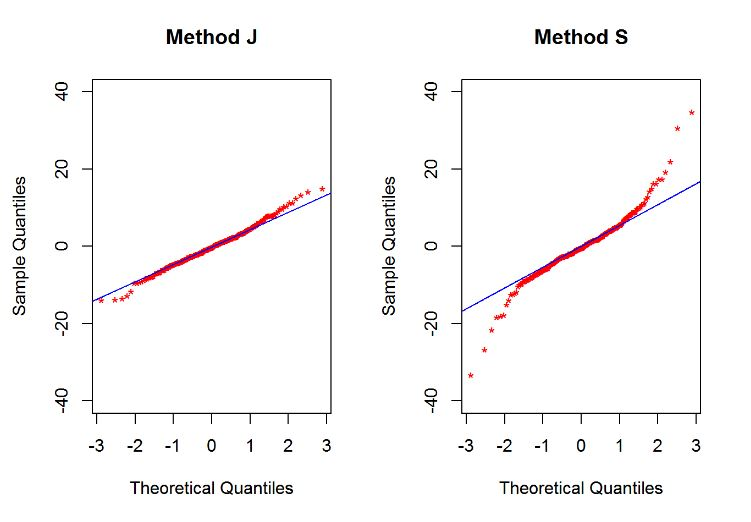
\includegraphics[width=1.1\linewidth]{images/Resid-newplot2}
%		\caption{}
%		\label{fig:Resid-newplot2}
%	\end{figure}
	
	
%	\begin{figure}[h!]
%		\centering
%		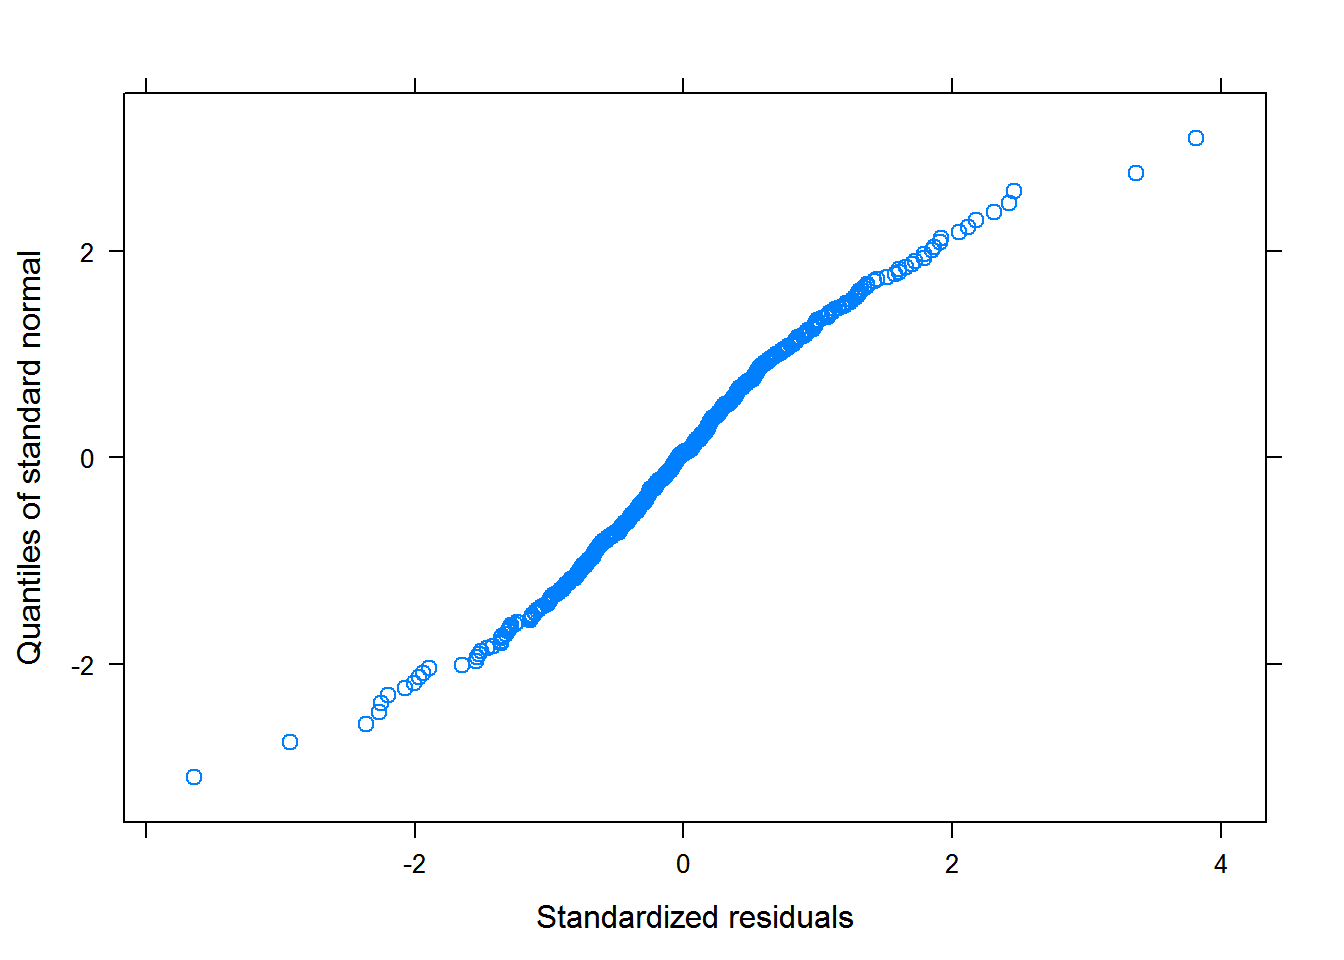
\includegraphics[width=0.9\linewidth]{images/ResidPlot3}
%		\label{fig:ResidPlot3}
%	\end{figure}
%	
%	
%	\begin{figure}[h!]
%		\centering
%		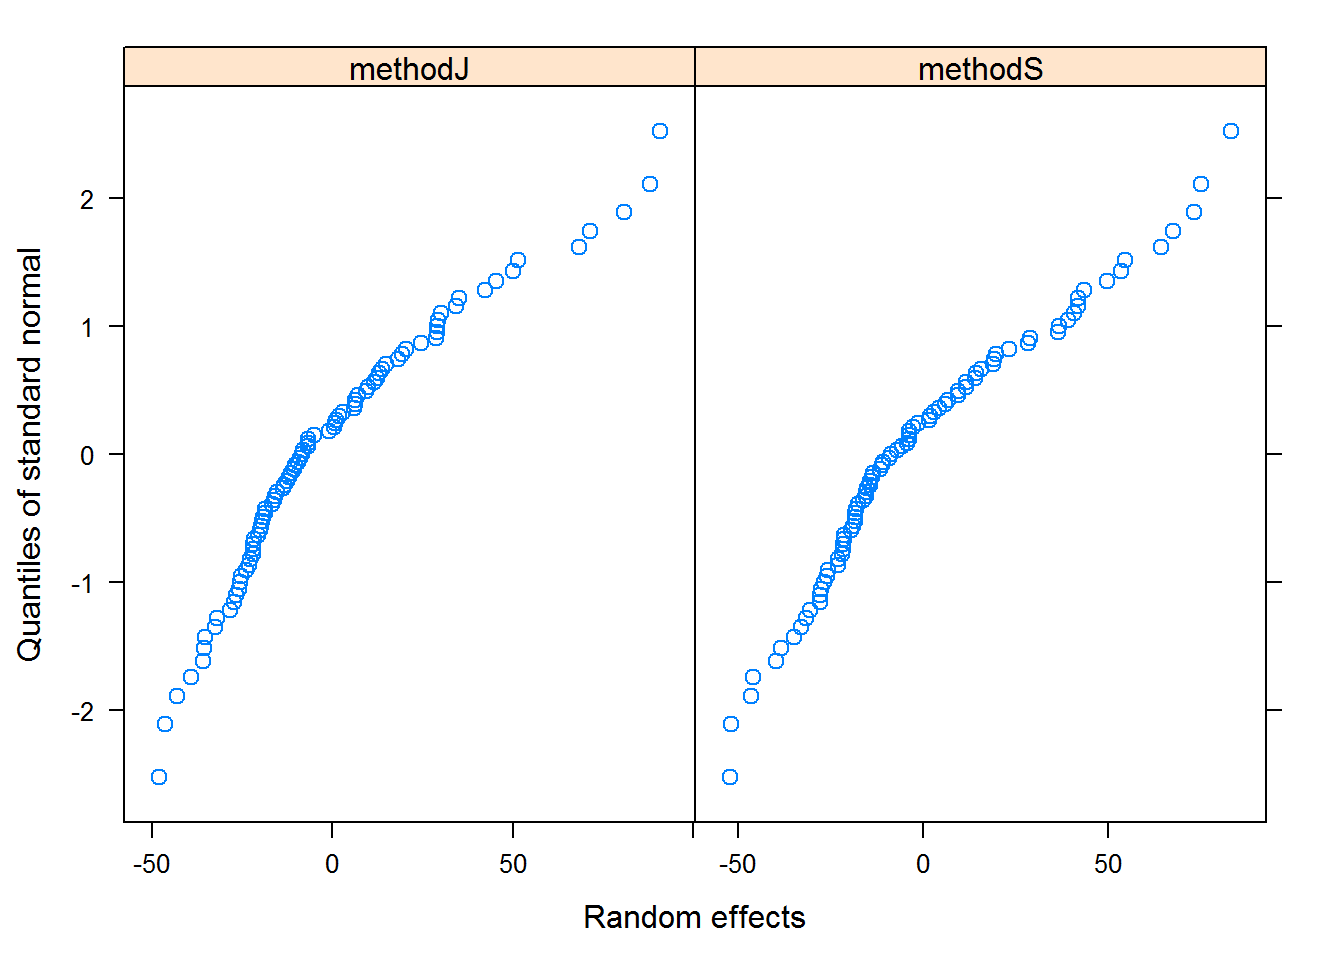
\includegraphics[width=0.9\linewidth]{images/ResidPlot2}
%		\caption{}
%		\label{fig:ResidPlot2}
%	\end{figure}
%
%	


%The fitted model used in the Blood data example, \texttt{JS.ARoy20091}, was fitted using the \texttt{lme()} function from the nlme package, and as such, is stored as an \texttt{lme} object. The \texttt{residual} functions extracts residuals of a fitted LME model, depending on the type of residual required.
%
%\begin{figure}[h!]
%	\centering
%	\includegraphics[width=0.9\linewidth]{images/Residuals-JS-roy}
%	\caption{}
%	\label{fig:Residuals-JS-ARoy2009}
%\end{figure}

	\subsubsection{Taxonomy of LME Residuals}
	Standard residual and influence diagnostics for linear models can
	be extended to linear mixed models. The dependence of
	fixed-effects solutions on the covariance parameter estimates has
	important ramifications in perturbation analysis. To gauge the
	full impact of a set of observations on the analysis, covariance
	parameters need to be updated, which requires refitting of the
	model.

\citet{PB} describes three types of residual that describe the variabilities
present in LME models
\begin{enumerate}
	\item marginal residuals, $\hat{\xi}$, which predict marginal errors,
	\item conditional residuals, $\hat{\epsilon}$, which predict conditional errors,
	\item the BLUP,$\boldsymbol{Z\hat{b}}$, that predicts random effects.
\end{enumerate}
Each type of residual is useful to evaluates some assumption of the model.
	%---http://www.stat.purdue.edu/~bacraig/notes598S/SUGI_Paper_Schabenberger.pdf
	
\citet{PB} describes three types of residual that describe the variabilities
present in LME models, marginal residuals, $\hat{\xi}$, which predict marginal errors, conditional residuals, $\hat{\epsilon}$, which predict conditional errors, and the BLUP,$\boldsymbol{Z\hat{b}}$, that predicts random effects.
Each type of residual is useful to evaluates some assumption of the model.
	
The definitions of both marginal residuals ($r_m$) and conditional residuals ($r_c$) follow from the definitions of marginal and conditional means in the LME model 
	$E[{Y}] = {X}{\beta}$ and $E[{Y|u}] = {X}{\beta} + {Z}{u}$, respectively.
	
A marginal residual is the difference between the observed data and the estimated marginal mean. A conditional residual is the difference between the observed data and the predicted value of the observation. In a model without random effects, both sets of residuals coincide.

The conditional (subject-specific) and marginal (population-averaged) formulations in the linear mixed model enable you to consider conditional residuals that use the estimated BLUPs of the random effects, and marginal residuals which are deviations from the overall mean. Residuals using the BLUPs are useful to diagnose whether the random effects components in the model are specified correctly, marginal residuals are useful to diagnose the fixed-effects components.	

The raw residuals $r_{mi}$ and $r_{ci}$ are usually not well suited for these purposes.
	
	
	%- http://www.ime.usp.br/~jmsinger/MAE5705/EMR2013.pdf
	
According to Hilton \& Minton (1995), a residual is considered pure for a specfic type fo error
	if it depends only on the fixed components and on the error that it is supposed to predict.
	Residuals that depend on other types of error are known as `confounded errors'.
	
	
The marginal raw residual is

\[ r_{Mar} = y - X \hat{\beta}. \]

	
	Conditional residuals include contributions from both fixed and random effects, whereas marginal residuals include contribution from only fixed effects.
	
Marginal residuals are good for checking fixed effects.	

	%In linear mixed effects models, diagnostic techniques may consider `conditional' residuals. A conditional residual is the difference between an observed value $y_{i}$ and the conditional predicted value $\hat{y}_{i} $.
	%
	%\[ \hat{epsilon}_{i} = y_{i} - \hat{y}_{i} = y_{i} - ( X_{i}\hat{beta} + Z_{i}\hat{b}_{i}) \]
	%

Conditional residuals include contributions from both fixed and random effects, whereas marginal residuals include contribution from only fixed effects. Marginal residuals should have mean of zero, but may show grouping structure. Also they may not be homoscedastic.

\subsubsection{Summary of Paper}

Standard residual and influence diagnostics for linear models can be extended to LME models. The dependence of the fixed effects solutions on the covariance parameters has important ramifications on the perturbation analysis. Calculating the studentized residual and influence statistics whereas each software procedure can calculate both conditional and marginal raw residuals, only SAS Proc Mixed is currently the only program that provide studentized residuals Which ave preferred for model diagnostics. The conditional raw residuals ave not well suited to detecting outliers as are the studentized conditional residuals \citep{schabenberger}.



LME are flexible tools for the analysis of clustered and repeated measurement data. LME extend the capabilities of standard linear models by allowing unbalanced and missing data, as long as the missing data are MAR. Structured covariance matrices for both the random effects G and the residuals R. 


\section{Influence Diagnostics}

	


	
Influential points have a large influence on the fit of the model. Influential points are a set of one or more observations whose removal would cause a different conclusion in the analysis, e.g. substantially changes the estimate of the regression coefficients. \citet{west} remarks that influence diagnostics play an important role in the interpretation of results, because influential data can negatively influence the statistical model and generalizability of the model. Influence diagnostics are formal techniques that allow the identification observation that heavily influence estimates of parameters.



Influence diagnostics are formal techniques that allow the identification observation that heavily influence estimates of parameters.
Influential points are a set of one or more observations whose removal would cause a different conclusion in the analysis, e.g. substantially affect estimates. \citet{west} remarks that influence diagnostics play an important role in the interpretation of results, because influential data can negatively influence the statistical model and generalizability of the model.



	%Influential points have a large influence on the fit of the model. 
	
	%One approach for determining influential points is to compare the fit of the model with and without each observation.
	
	%The basic rationale behind identifying influential data is that when iteratively single units are omitted from the data, models based on these data should not produce substantially different estimates. 
Influence can be thought of as consequence of leverage and outlierness. Outliers are the most noteworthy data points in an analysis, and an objective of influence analysis is how influential they are, and the manner in which they are influential. They can point to a model breakdown and lead to development of a better model.

LME model are a useful framework for fitting a wide range of models. However, they are known to be sensitive to outliers. Specifically likelihood based estimation techniques, such as ML and REML, are sensitive to outliers. \citet{Christensen} advises that identification of outliers is necessary before conclusions may be drawn from the fitted model. The leverage of an observation is a further consideration. 
	
%An observation with an extreme, but not unusual, value on a predictor variable is a point with high leverage. High leverage points can have a great amount of effect on the estimate of regression coefficients. In general. a high leverage point means a extreme value for the one or more of the independent variables, and a greater potential of overly influencing the final fitted model. However, if a case has  extreme values for the independent variables but is fitted very well by a regression model, this case is not necessarily overly influential.

	


\subsection{Cook's Distance}

\index{Cook's Distance} Cooks Distance ($D_{i}$) is a diagnostic technique used in classical linear models, that functions as an overall measure of the influence of an observation that is a measure of aggregate impact of each observation on the group of regression coefficients, as well as the group of fitted values. \index{Cook's distance} Cook's Distance as a measure of the influence of observations in subset $U$ on a vector of parameter estimates is given below \citep{cook77}
\[ \delta_{(U)} = \hat{\beta} - \hat{\beta}_{(U)}.\]
Observations, or sets of observations, that have high Cook's distance usually have high residuals, although this is not necessarily the case.


If the predictions are the same with or without the observation in question, then the observation has no influence on the regression model. If the predictions differ greatly when the observation is not included in the analysis, then the observation is influential.

Large values for Cook's distance indicate observations for special attention. Cook's distance can be used in several ways: to indicate data points that are particularly worth checking for validity; to indicate regions of the design space where it would be good to be able to obtain more data points.

Use of threshold values for Cook's Distance is discouraged \citep{fox1991}. However, informal heuristics do exist for OLS models, with an informal threshold of $4/n$ or $4/(n-k-1)$, where $n$ is the number of observations and $k$ the number of explanatory variables.

\citet{fox1991} advises the use of diagnostic plotting and to examine in closer details the points with \textit{``values of D that are substantially larger than the rest}", and that thresholds should feature only to enhance graphical displays.

The effect on the precision of estimates is separate from the effect on the point estimates. Data points that have a small \index{Cook's distance}Cook's distance, for example, can still greatly affect hypothesis tests and confidence intervals, if their  influence on the precision of the estimates is large.

\citet{Christensen} develops \index{case deletion diagnostics} case deletion diagnostics, in particular the equivalent of \index{Cook's distance} Cook's distance for diagnosing influential observations when estimating the fixed effect parameters and variance components, adapting the \index{Cook's distance}Cook's Distance measure for the analysis of LME models. For LME models, two formulations exist; a \index{Cook's distance}Cook's distance that examines the change in fixed fixed parameter estimates, and another that examines the change in random effects parameter estimates. The outcome of either Cook's distance is a scaled change in either $\beta$ or $\theta$. \citet{Zewotir} gives a detailed discussion of the various formulation for Cook's distances for LME Models.

	
%	For LME models, Cook's distance can be extended to model influence diagnostics by defining:
%	\[ C_{\beta i} = {(\hat{\beta} - \hat{\beta}_{[i]})^{T}(\boldsymbol{X}^{\prime}\boldsymbol{V}^{-1}\boldsymbol{X}) (\hat{\beta} - \hat{\beta}_{[i]}) \over p}\]
%	
%	It is also desirable to measure the influence of the case deletions on the covariance matrix of $\hat{\beta}$.

%	It uses the same structure for measuring the combined impact of the differences in the estimated regression coefficients when the $i$th case is deleted. Importantly, $D_{(i)}$ can be calculated without fitting a new regression coefficient each time an observation is deleted.

%Cook's Distance is proportional to the sum of the squared differences between predictions made with all observations in the analysis and predictions made leaving out the observation in question.



Consideration of how leave-$U$-out diagnostics would work in the context of Method Comparison problems is required. There are several scenarios. \citet{preisser} describes two type of diagnostics. When the set consists of only one observation, the type is called
`\textit{observation-diagnostics}'. For multiple observations, Preisser describes the diagnostics as `\textit{cluster-deletion}' diagnostics. Suppose we have two methods of measurement X and Y, each with three measurements for a specific case: $(x_1,x_2,x_3,y_1,y_2,y_3)$

\begin{itemize}
	\item Leave One Out - one observation is omitted (e.g. $x_1$)
	\item Leave Pair Out - one pair of observation  is omitted (e.g. $x_1$ and $y_1$)
	\item Leave Case (or Item or Subject) Out - All observations associated with a particular case or subject are omitted. (e.g. $\{x_1,x_2,x_3,y_1,y_2,y_3\}$)
\end{itemize}
%% Schabenberger

The natural sampling unit is the item or subject, similar to the example provided by \citet{schabenberger}. Hence, the third option, henceforth, referred to as ``Leave subject Out" will be the option used.

	
	
	\begin{figure}[h!]
		\centering
		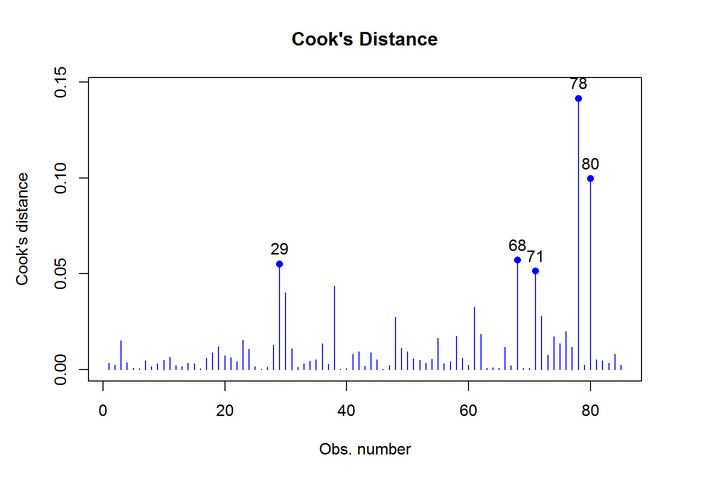
\includegraphics[width=0.9\linewidth]{images/CooksDistancePlot-JS-Roy}
		\caption{}
		\label{fig:CooksDistancePlot-JS-Roy}
	\end{figure}	
	%	For LME models, Cook's distance can be extended to model influence diagnostics by defining:
	%	\[ C_{\beta i} = {(\hat{\beta} - \hat{\beta}_{[i]})^{T}(\boldsymbol{X}^{\prime}\boldsymbol{V}^{-1}\boldsymbol{X}) (\hat{\beta} - \hat{\beta}_{[i]}) \over p}\]
	%	
	%	It is also desirable to measure the influence of the case deletions on the covariance matrix of $\hat{\beta}$.
	


	



	\section{Model Diagnostics for Roy's Models}
	
	Further to previous work, this section revisits case-deletion and residual diagnostics, and explores how approaches devised by  \citet{Galecki} can be used to appraise Roy's model. These authors specifically look at Cook's Distances and Likelihood Distances.
	%	For the Roy Model, Cook's Distances may also be generated using the \textbf{\textit{predictmeans}}
	%	
	
	
	
	
	
	\begin{figure}[h!]
		\centering
		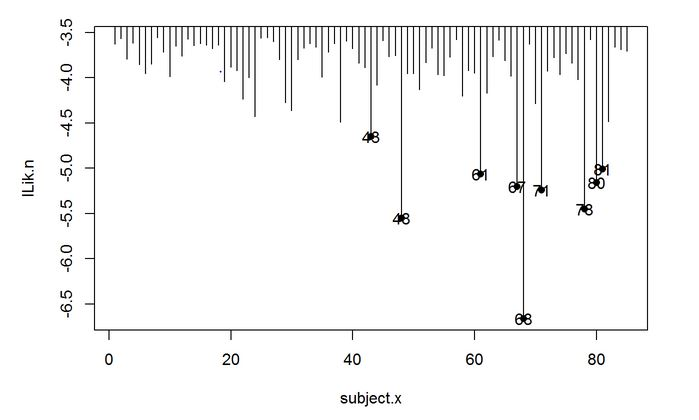
\includegraphics[width=0.7\linewidth]{images/LogLik-JS-Roy}
		\caption{}
		\label{fig:LogLik-JS-Roy}
	\end{figure}
	
	
	
\subsection{Deletion Diagnostics}
	
	%Data from single individuals, or a small group of subjects may influence non-linear mixed effects model selection. 
	%Diagnostics routinely applied in model building may identify such individuals, but these methods are not specifically designed for that purpose and are, therefore, not optimal. 
	%We describe two likelihood-based diagnostics for identifying individuals that can influence the choice between two competing models.
	
	
	Deletion diagnostics provide a means of assessing the influence of an observation (or groups of observations) on parameters inferences for a fitted model. For classical linear models, \citet{cook77} greatly expands the study of residuals and influence measures. The key to making deletion diagnostics useable is the development of efficient computational formulas, allowing one to obtain the \index{case deletion diagnostics} case deletion diagnostics by making use of basic building blocks, computed only once for the full model.
	Cook's key observation was the effects of deleting each observation in turn could be calculated with little additional computation. Cook proposed a measure that combines the information of leverage and residual of the observation, now known simply as the Cook's Distance, $D_{(i)}$, which can be calculated without fitting a new regression coefficient each time an observation is deleted. Consequently deletion diagnostics have become an integral part of assessing linear models.
	
	
	
	It must be pointed out that the effect on the precision of estimates is separate from the effect on the point estimates. Data points that have a small \index{Cook's distance}Cook's distance, for example, can still greatly affect hypothesis tests and confidence intervals, if their 
	influence on the precision of the estimates is large.	
	
	\citet{Christensen} notes the case deletion diagnostics techniques have not been applied to linear mixed effects models and seeks to develop methodologies in that respect. \citet{Christensen} developed their global influences for the deletion of single observations in two steps: a one-step estimate for the REML (or ML) estimate of the variance components, and an ordinary case-deletion diagnostic for a weighted resgression problem (conditional on the estimated covariance matrix) for fixed effects.
	
	The computation of case deletion diagnostics in the classical model is made simple by the fact that estimates of $\beta$ and $\sigma^2$, which exclude the $i$th observation, can be computed without re-fitting the model. Such update formulas are available in the mixed model only if you assume that the covariance parameters are not affected by the removal of the observation in question. This is rarely a reasonable assumption, and undermines the use of many proposed procedures for method comparison.



\section{Using DFBETAs from LME Models to Assess Agreement}

The impact of an observation on a regression fitting can be determined by the difference between the estimated regression coefficient of a model with all observations and the estimated coefficient when the particular observation is deleted. DFBETA and DFFITS are well known measures of influence. Emphasis shall be placed on DFBETA, but a brief discussion of DFFITS is merited as it potentially provides for useful techniques in method comparison. \citet{schabenberger} provides a mathematical desciption of both.

DFBETAS is a standardized measure of the absolute difference between the estimate with a particular
case included and the estimate without that particular case,, thus measuring the impact each observation has on a particular predictor \citep{belsley2005}. For LME models, the DFBETA is a measure that standardizes the absolute difference in parameter estimates between an LME model based on a full set of data, and a model from reduced data.

In general, large values of DFBETAS indicate observations that are influential in estimating a given parameter. There is no agreement as to the critical threshold for DFBETAs. \citet{belsleywelsch} recommend 2 as a general cutoff value to indicate influential observations and as a size-adjusted cutoff.  The cut-off value for DFBETAs is $\frac{2}{\sqrt{n}}$, where $n$ is the number of observations. 
%However, another cut-off is to look for observations with a value greater than 1.00. Here cutoff means,
%``this observation could be overly influential on the estimated coefficient".







\bibliography{2017bib}

	

\end{document}


%---------------------------------------------------------------------------------------------------%


